%%%%%%%%%%%%%%%%%%%%%%%%%%%%%%%%%%%%%%%%%%%%%%%%%%%%%%%%%%%%%%%%%%%%%%
% Problem statement
\begin{statement}[
  problempoints=50,
  timelimit=1 second,
  memorylimit=512 MiB,
]{Datum}

\setlength\intextsep{-0.1cm}
\begin{wrapfigure}[6]{r}{0.22\textwidth}
\centering
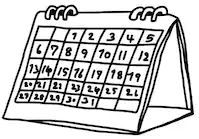
\includegraphics[width=0.22\textwidth]{img/datum.png}
\end{wrapfigure}

The exam season at University of Zagreb is over and students are doing what
they love the most -- sleeping. In the rare moments of wakefulness, they usually
scroll over their Instagram feed. Fabijan is one of those students.

Recently, he read the following caption -- the date \texttt{02.02.2020.} is
the first palindromic date in the last $909$ years.

He realized the caption was incorrect and this made him wonder about
palindromic dates so he asked himself for each of the $N$ dates what is the
first palindromic date that comes after that date.  The date is considered
\textit{palindromic} if
  , when disregarding the dots, it is the same when read
from left-to-right as if it was read from right-to-left.  For example, dates
\texttt{02.02.2020.} and \texttt{12.10.0121.} are palindromic, while
\texttt{03.02.2020.} and \texttt{12.07.1993.} are not.

\textbf{Note:} In this task it is important to take account of leap years
which have $29$ days in February. For the purposes of this task, we consider
a year to be a leap year if it is divisible by $4$. Otherwise, months have
$31$, $28$, $31$, $30$, $31$, $30$, $31$, $31$, $30$, $31$, $30$ and $31$ days
in order.

%%%%%%%%%%%%%%%%%%%%%%%%%%%%%%%%%%%%%%%%%%%%%%%%%%%%%%%%%%%%%%%%%%%%%%
% Input
\subsection*{Input}
The first line contains an integer $N$ $(1 \le N \le 10\ 000)$ from the task
description.

The next $N$ lines contain a valid date in format \texttt{DD.MM.YYYY.}

%%%%%%%%%%%%%%%%%%%%%%%%%%%%%%%%%%%%%%%%%%%%%%%%%%%%%%%%%%%%%%%%%%%%%%
% Output
\subsection*{Output}
For each date from the input, you should output the first palindromic date that
comes strictly after it. That date should be printed in the \texttt{DD.MM.YYYY.}
and we guarantee that the solution exists in this format.

%%%%%%%%%%%%%%%%%%%%%%%%%%%%%%%%%%%%%%%%%%%%%%%%%%%%%%%%%%%%%%%%%%%%%%
% Scoring
\subsection*{Scoring}
In the test cases worth a total of $10$ points, each date in the output will
have the same month and year as the corresponding date from the input. Also,
$N$ will be equal to $10$.

In the test cases worth an additional $10$ points, each date in the output will
have the same year as the corresponding date from the input. Also, $N$ will
be equal to $10$.

In the test cases worth an additional $20$ points, $N=10$ will hold.

%%%%%%%%%%%%%%%%%%%%%%%%%%%%%%%%%%%%%%%%%%%%%%%%%%%%%%%%%%%%%%%%%%%%%%
% Examples
\subsection*{Examples}
\begin{tabularx}{\textwidth}{X'X'X}
\sampleinputs{test/datum.dummy.in.1}{test/datum.dummy.out.1} &
\sampleinputs{test/datum.dummy.in.2}{test/datum.dummy.out.2} &
\sampleinputs{test/datum.dummy.in.3}{test/datum.dummy.out.3}
\end{tabularx}

\textbf{Clarification of the first example:}
Although the given date is palindromic, Fabijan is interested in the first
date that strictly comes after it. That date is \texttt{12.02.2021.}

%%%%%%%%%%%%%%%%%%%%%%%%%%%%%%%%%%%%%%%%%%%%%%%%%%%%%%%%%%%%%%%%%%%%%%
% We're done
\end{statement}

%%% Local Variables:
%%% mode: latex
%%% mode: flyspell
%%% ispell-local-dictionary: "croatian"
%%% TeX-master: "../hio.tex"
%%% End:
